%!TEX root =  ../main.tex
%\thispagestyle{empty}
\renewcommand{\columnseprule}{1.5pt}
\begin{multicols*}{2}
\noindent
\rule[0.5\baselineskip]{0.5\textwidth}{1pt}
\noindent
\subsection{Through the Looking Glass}
\noindent
1. In the four, blank squares below, fill in the correct sign (positive or negative) of the answer.
Take a number of the sign given on the left to a power of the kind given above.  For example, 
top-left square is asking for the sign of a positive number to an even power (e.g. $31^{60}$ is positive).

\noindent
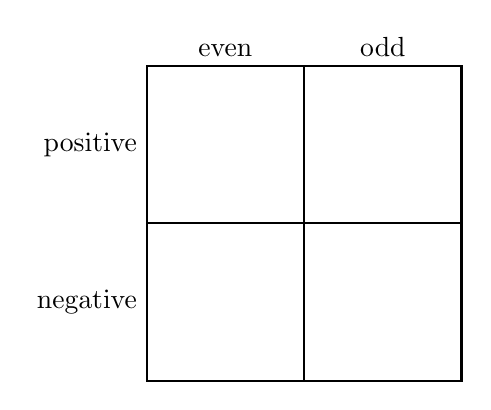
\begin{tikzpicture}
	\draw [thick,-] (0,0) -- (4,0) -- (4,4) -- (0,4) -- cycle;
	\draw [thick,-] (2,0) -- (2,4);
	\draw [thick,-] (0,2) -- (4,2);
	\draw (0,1) node[anchor=east] {negative};
	\draw (0,3) node[anchor=east] {positive};
	\draw (1,4) node[anchor=south] {even};
	\draw (3,4) node[anchor=south] {odd};
\end{tikzpicture}

\vspace{0.2cm}

\noindent
2. Sketch the graph $y=x^2$ without using a graphing calculator.  Leave $x$ 1:1, but scale 
the $y$-values 1:10.

\noindent
\begin{centering}
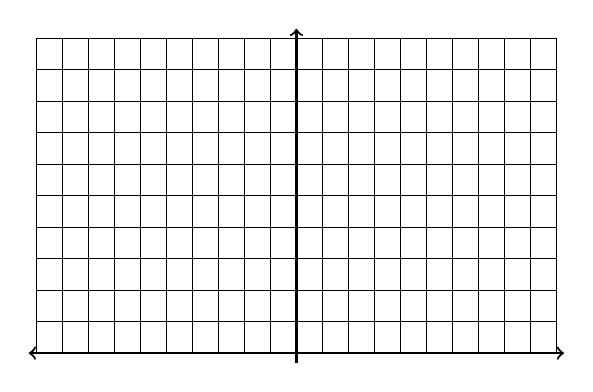
\begin{tikzpicture}[xscale=0.33,yscale=0.04]
	\draw [thick, <->] (-10.3,0) -- (10.3,0);
	\draw [thick, ->] (0,-3) -- (0,103);
	\draw [thin,ystep=10] (-10,0) grid (10,100);
\end{tikzpicture}
\end{centering}

\vspace{0.2cm}

\noindent
3. On the same graph above, graph $y=x^4$, $y=x^6$, and $y=x^8$.  Do not use the graphing
function of your calculator!

\vspace{0.2cm}

\noindent
4. Continue not to use a graphing aide and stick to the same scale, but on the graph at the top of the next column, plot $y=x^3$.
 
\vspace{0.2cm}

\noindent
5. On the same graph with the cubic equation, add $y=x^5$, $y=x^7$, and the very
easy $y=x^1$.

\vspace{0.2cm}

\noindent
6. In technical language, describe the two different symmetries displayed by \textbf{even} powers of
$x$ and \textbf{odd} powers of $x$. 

\vspace{2.7cm}
~~~

\noindent
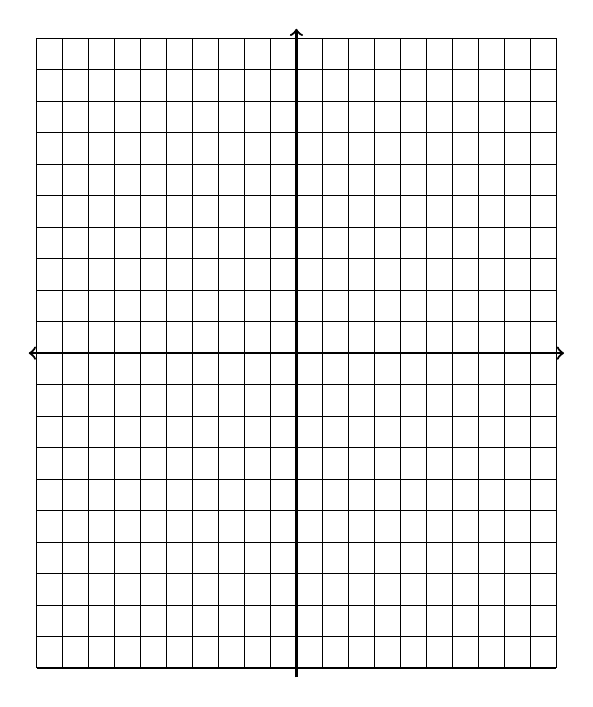
\begin{tikzpicture}[xscale=0.33,yscale=0.04]
	\draw [thick, <->] (-10.3,0) -- (10.3,0);
	\draw [thick, ->] (0,-103) -- (0,103);
	\draw [thin,ystep=10] (-10,-100) grid (10,100);
\end{tikzpicture}





\vspace{0.5cm}
\noindent
7. Next, create two algebra sentences for the two symmetries, each
in the form $f(x)=...f(-x)$.

\vspace{2cm}

\noindent
8. Do an image search on the internet for ``natural symmetry''.  Classify what you find as odd, or
even, or rotational.  Taking odd and rotational together and contrasting them with even, 
which kind(s) do you see as more \textit{human} than the other?  Why do you think that is?


\vspace{5cm}
\noindent
9. Describe what you think the point of this problem set is, using technical vocabulary in complete
sentences.
\end{multicols*}
